\section{The Parameter for GAN Structure}

\begin{figure*}
	\centering
	\begin{subfigure}{\linewidth}
		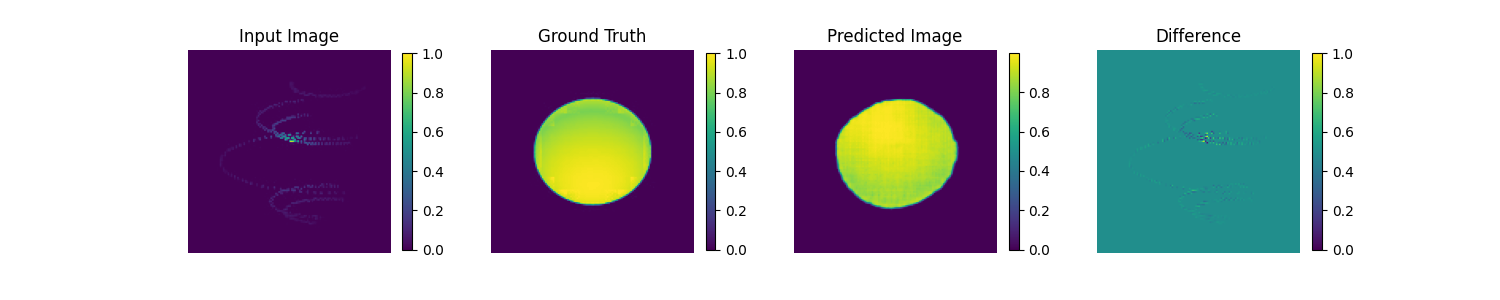
\includegraphics[width=\linewidth]{fig/testing_image/image_0.png}
	\end{subfigure}
	\begin{subfigure}{\linewidth}
		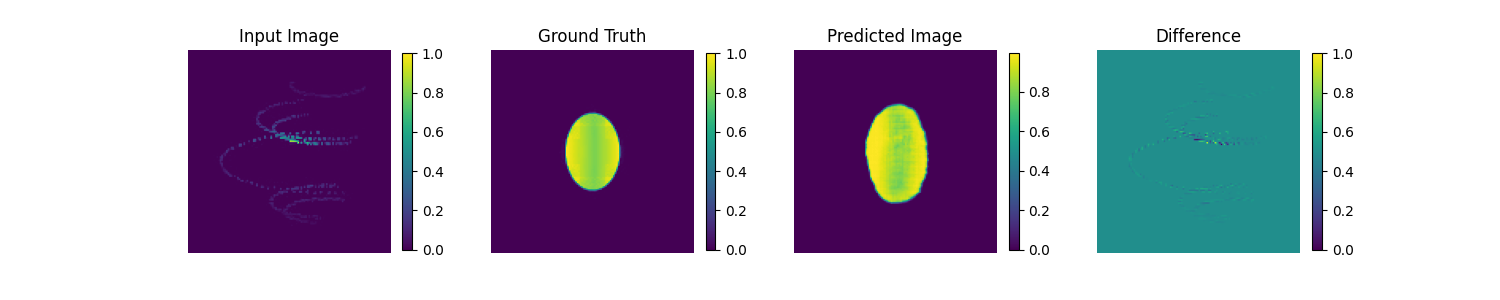
\includegraphics[width=\linewidth]{fig/testing_image/image_16.png}
	\end{subfigure}
	\begin{subfigure}{\linewidth}
		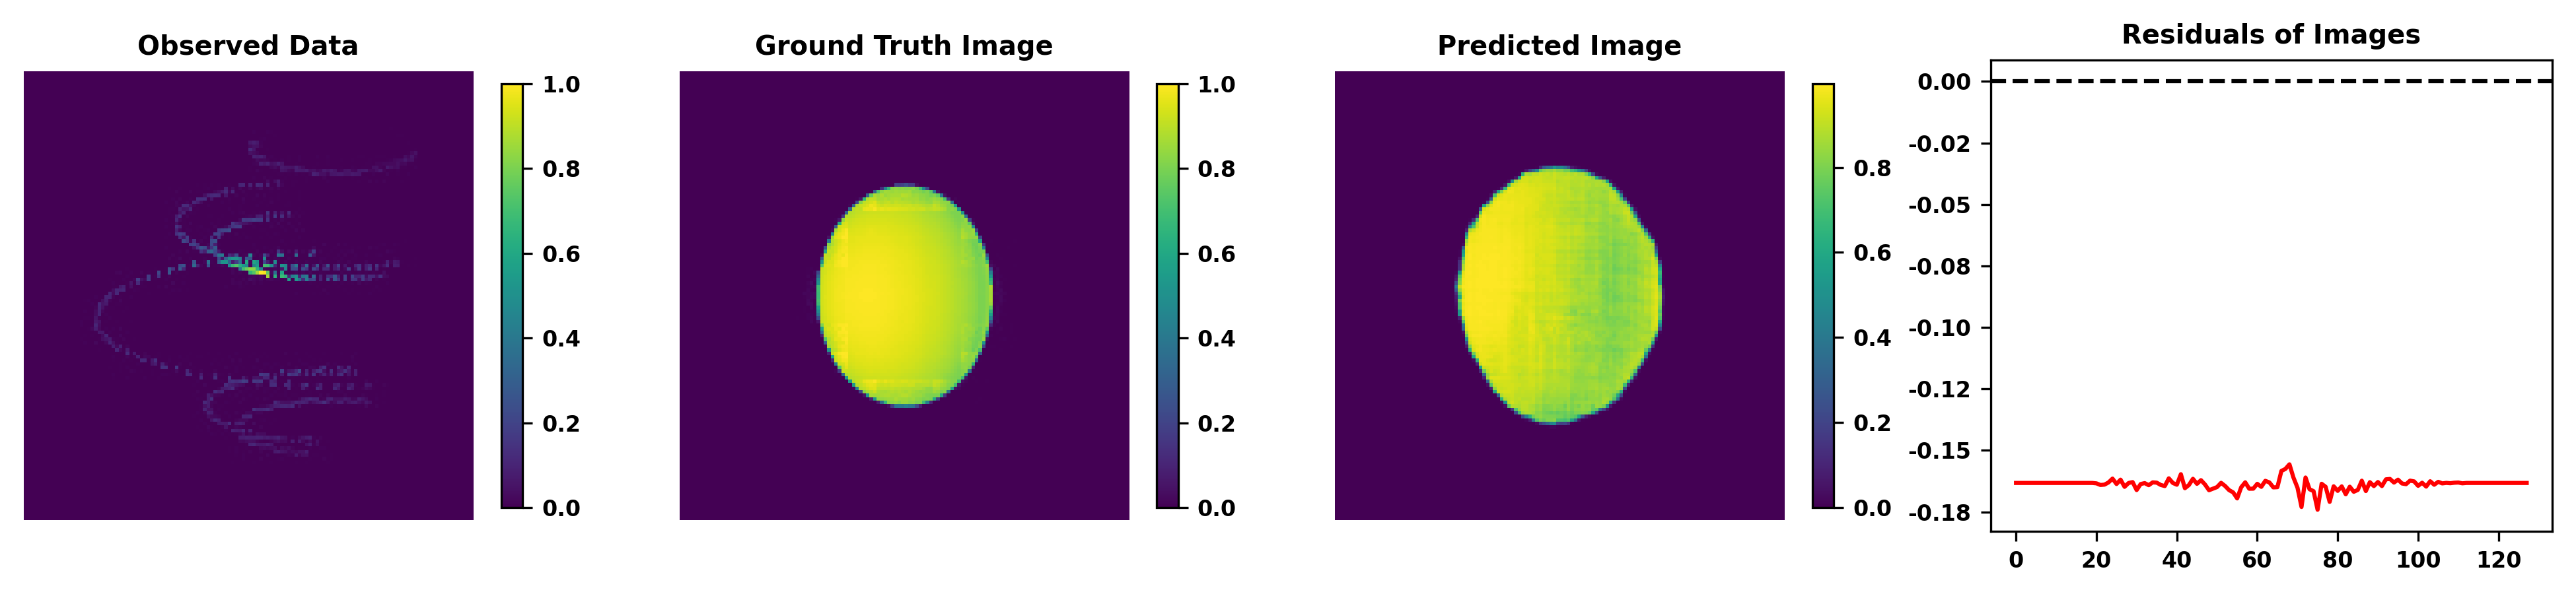
\includegraphics[width=\linewidth]{fig/testing_image/image_35.png}
	\end{subfigure}
	\begin{subfigure}{\linewidth}
		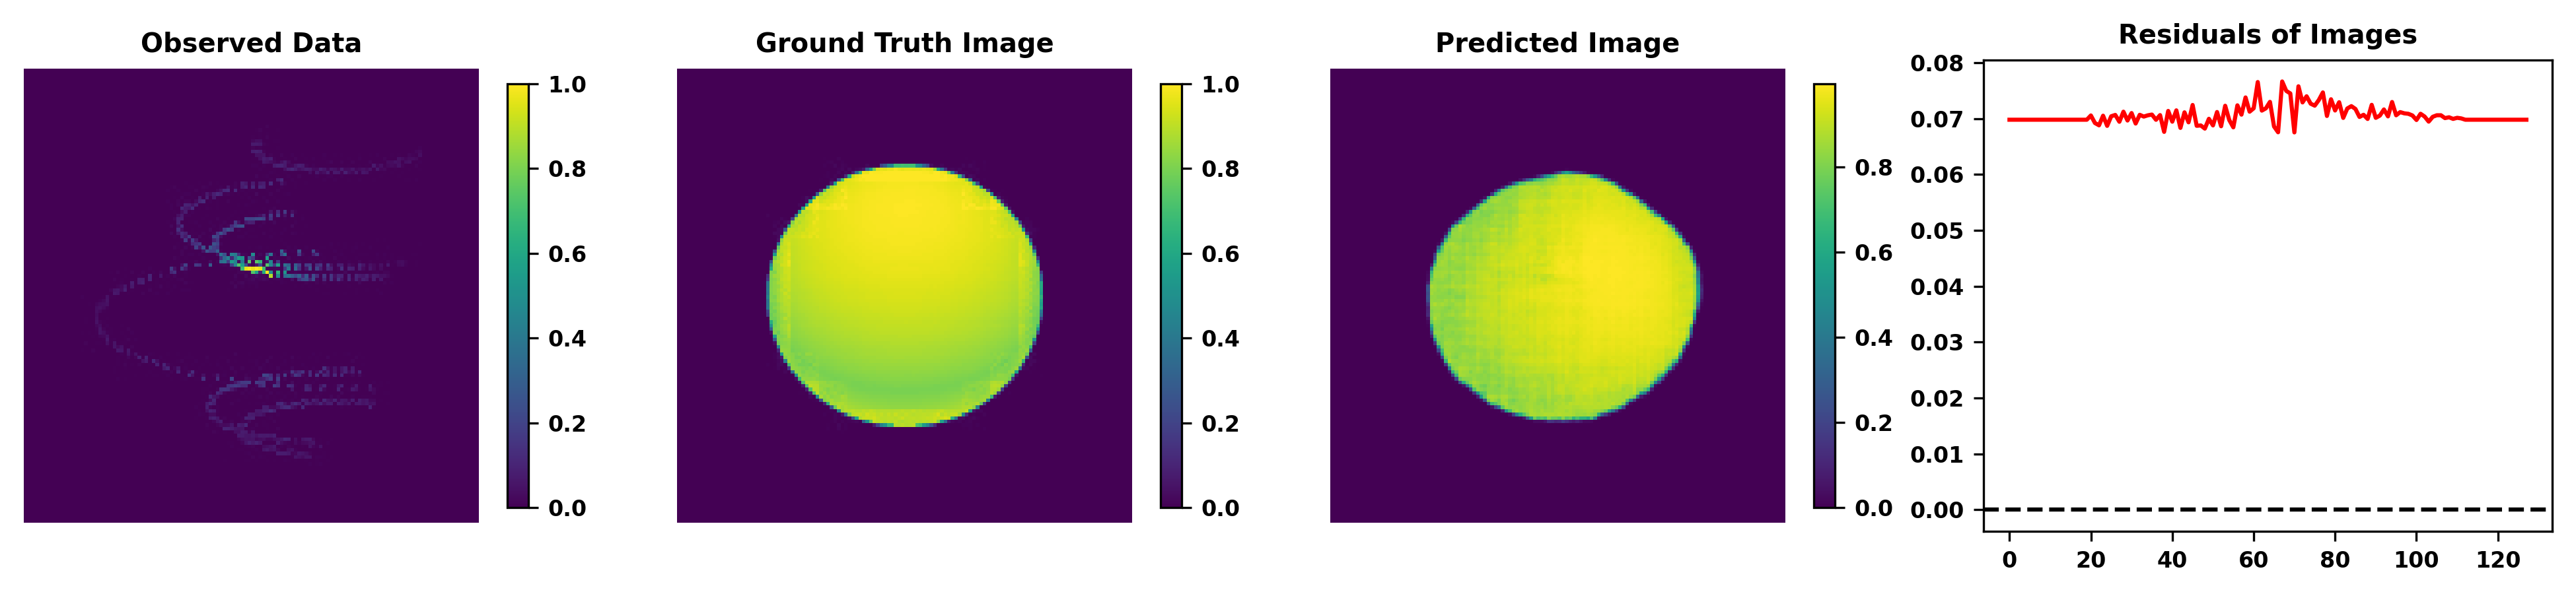
\includegraphics[width=\linewidth]{fig/testing_image/image_38.png}
	\end{subfigure}
	\begin{subfigure}{\linewidth}
		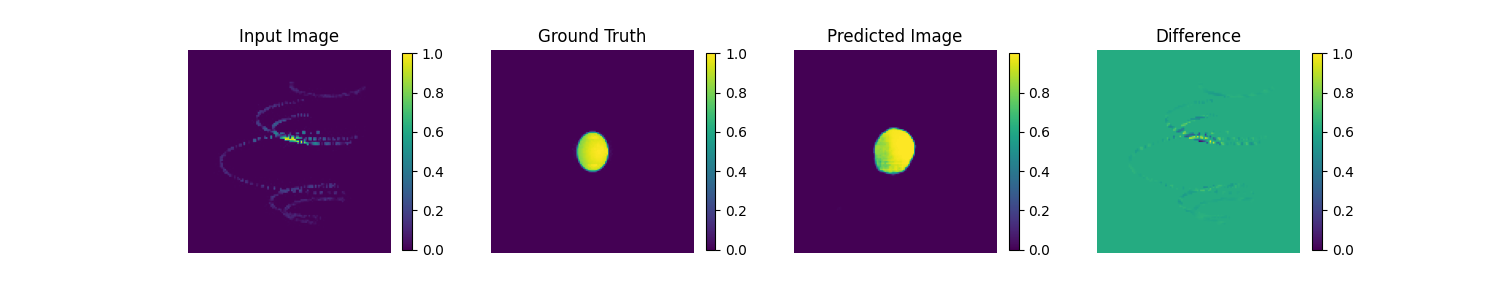
\includegraphics[width=\linewidth]{fig/testing_image/image_42.png}
	\end{subfigure}
	\begin{subfigure}{\linewidth}
		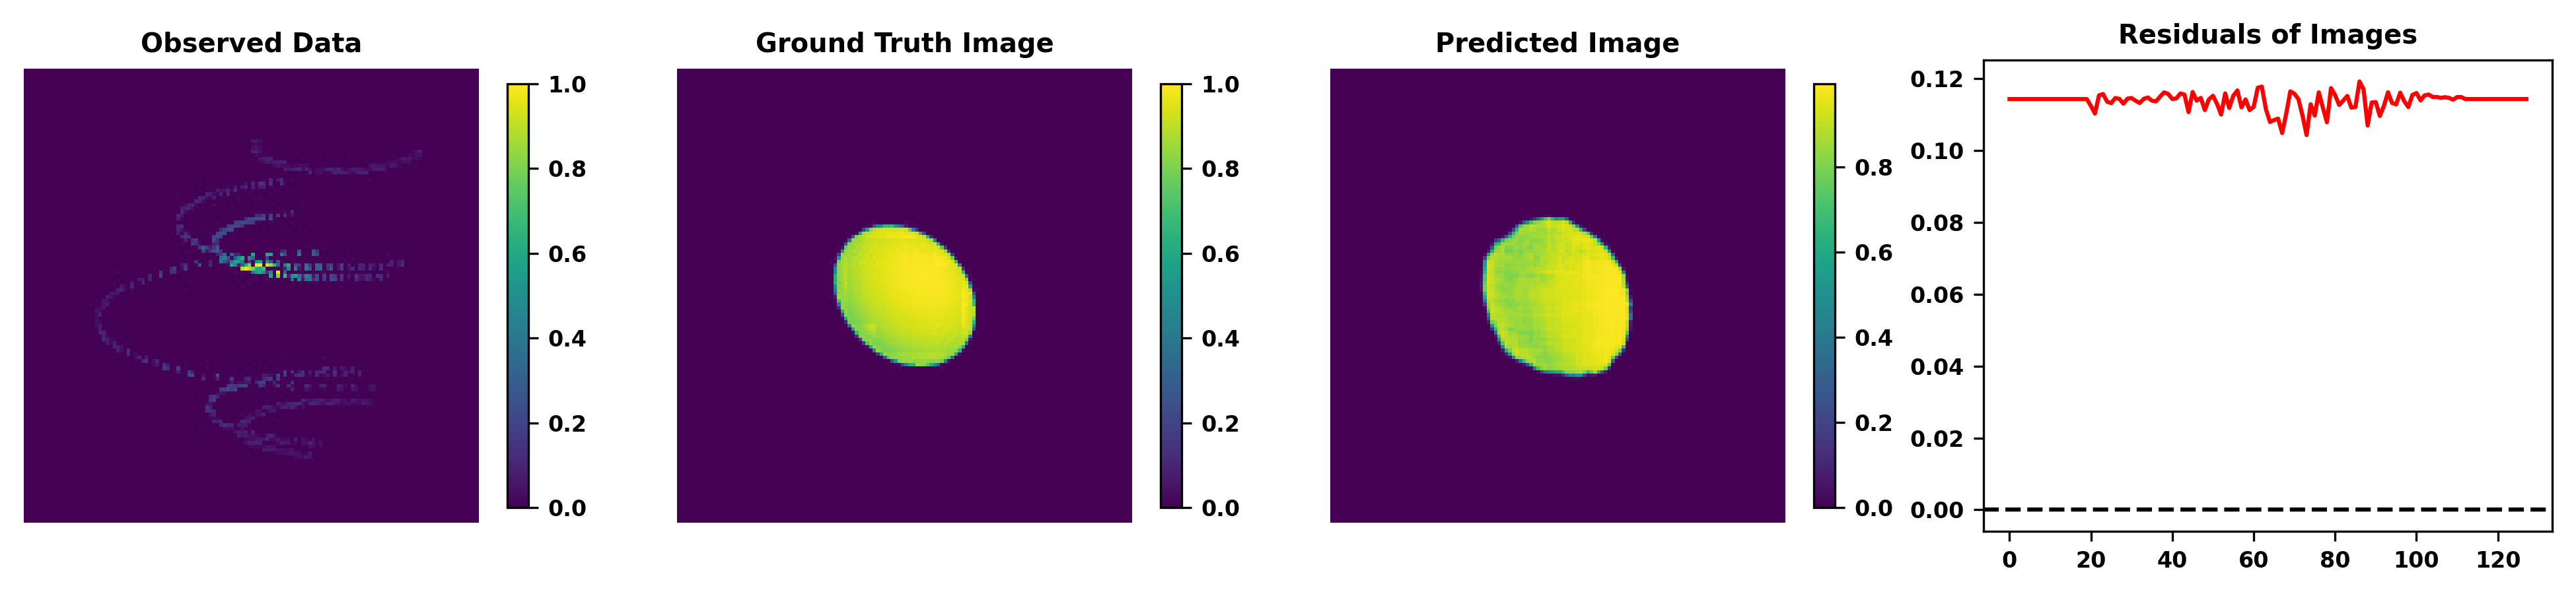
\includegraphics[width=\linewidth]{fig/testing_image/image_47.png}
	\end{subfigure}
	\caption{This set of figures shows the result of GAN for II. The left panels are signals using six baselines, which work as input for GAN. The first middle panel is the real image, also called ground truth, and GAN tries to mimic it during the training. The second middle panel is the reconstructed image, also called the predicted image, with trained GAN, and the end panel is the difference between the ground truth and the predicted image.}
	\label{fig:GAN}
\end{figure*}
Here, we discuss the parameters of the GAN architecture used for reconstructing images of stellar objects using II. Given the adversarial nature of GANs—where the Generator and Discriminator engage in a min-max game—careful tuning of key parameters is critical to ensure that both networks are well-balanced for effective training.

\subsection{Data Preparation}
First, we simulate fast-rotating stars, modeling them as oblate spheroids with varying radii and an oblateness ranging between 0.5 and 1. We also consider different viewing angles, assuming a linear dependence for the effect of gravity darkening. The traced ellipses result from integrating over the source's hour angle. For hyperparameter tuning and comparing different telescopes, the total hour angle is set to approximately 11.5 hours. Finally, the ellipses are plotted, converted into grayscale images, resized, and stored as raw arrays to facilitate further analysis.
\begin{figure*}
	\centering
	\begin{subfigure}{0.33\linewidth}
		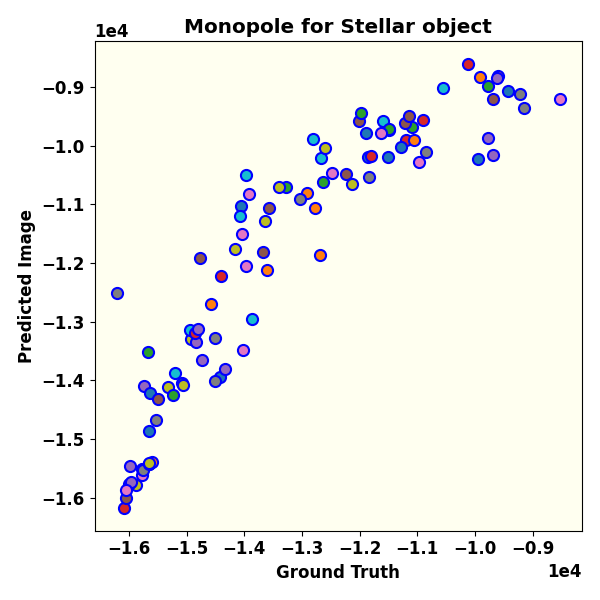
\includegraphics[width=\linewidth]{fig/moments/mom0.png}
		\caption{The monopole.}
		\label{fig:mom1}
	\end{subfigure}\hfill
	\begin{subfigure}{0.33\linewidth}
		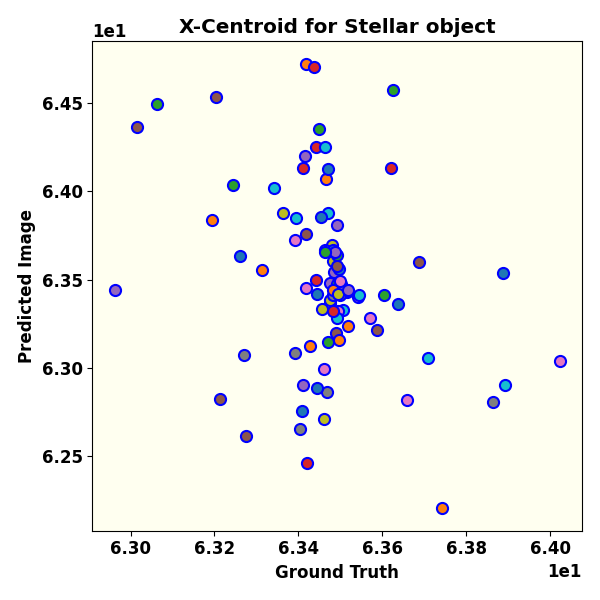
\includegraphics[width=\linewidth]{fig/moments/mom1.png}
		\caption{The centroids along x direction.}
		\label{fig:mom2}
	\end{subfigure}\hfill
	\begin{subfigure}{0.33\linewidth}
		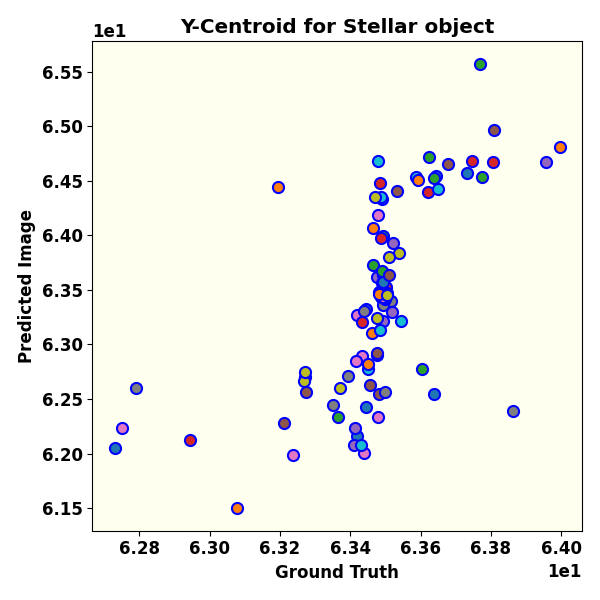
\includegraphics[width=\linewidth]{fig/moments/mom2.png}
		\caption{The centroids along y direction.}
		\label{fig:mom3}
	\end{subfigure}\hfill
	\caption{This set of figures shows the comparison of monopole, x-centroid, and y-centroid for ground truth and predicted images generated by trained GAN.}
	\label{fig:cen}
\end{figure*}
\begin{figure*}
	\centering
	\begin{subfigure}{0.33\linewidth}
		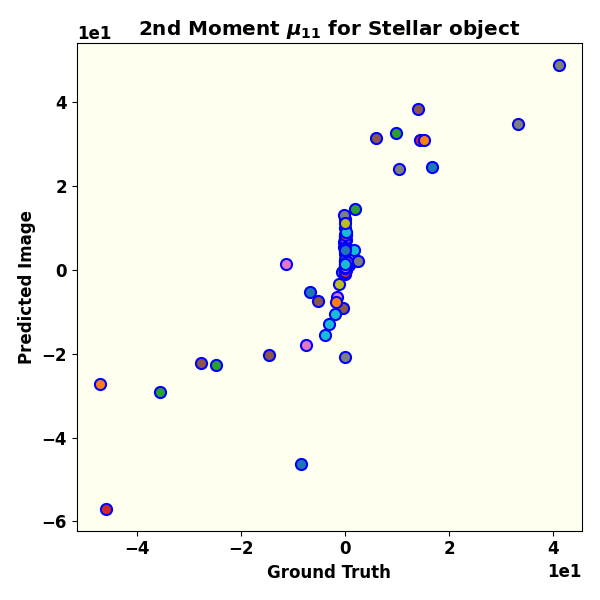
\includegraphics[width=\linewidth]{fig/moments/mom3.png}
		\caption{The 2nd order moment $\mu_{11}$.}
		\label{fig:mom4}
	\end{subfigure}\hfill
	\begin{subfigure}{0.33\linewidth}
		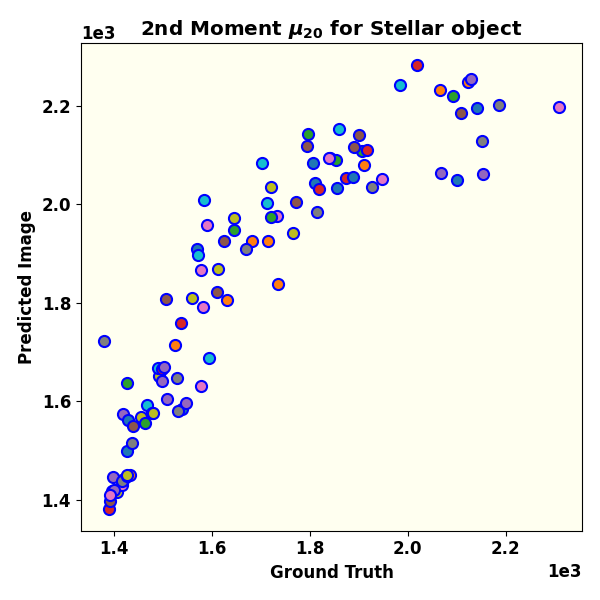
\includegraphics[width=\linewidth]{fig/moments/mom4.png}
		\caption{The 2nd order moment $\mu_{20}$.}
		\label{fig:mom5}
	\end{subfigure}\hfill
	\begin{subfigure}{0.33\linewidth}
		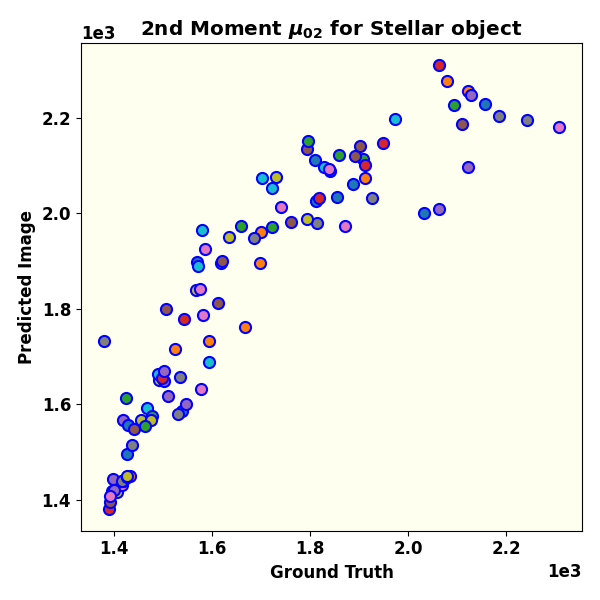
\includegraphics[width=\linewidth]{fig/moments/mom5.png}
		\caption{The 2nd order moment $\mu_{02}$.}
		\label{fig:mom6}
	\end{subfigure}\hfill
	\caption{The second-order central moments provide information about the size and shape of stellar objects. This set of figures shows all the second-order central moments for ground truth and predicted images generated by trained GAN.}
	\label{fig:struc}
\end{figure*}
\begin{figure*}
	\centering
	\begin{subfigure}{0.50\linewidth}
		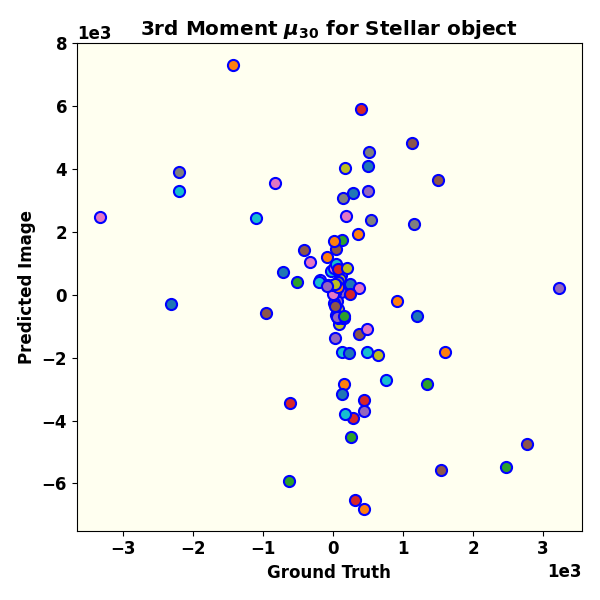
\includegraphics[width=\linewidth]{fig/moments/mom6.png}
		\caption{The 3rd order moment $\mu_{30}$.}
		\label{fig:mom7}
	\end{subfigure}\hfill
	\begin{subfigure}{0.50\linewidth}
		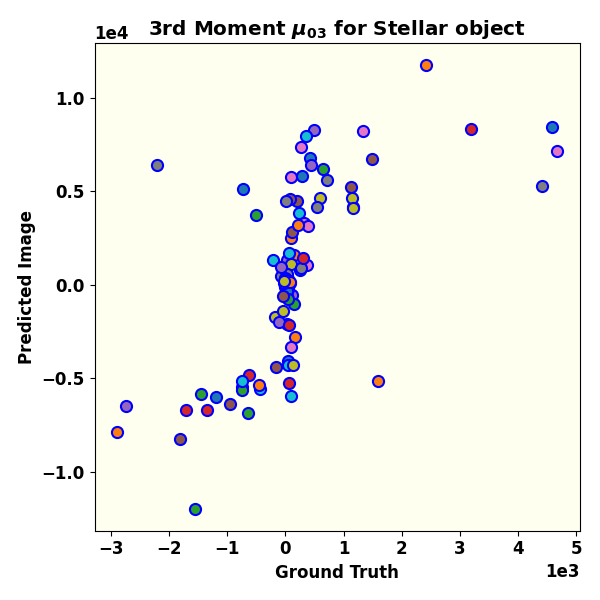
\includegraphics[width=\linewidth]{fig/moments/mom7.png}
		\caption{The 3rd order moment $\mu_{03}$.}
		\label{fig:mom8}
	\end{subfigure}\hfill
	\begin{subfigure}{0.50\linewidth}
		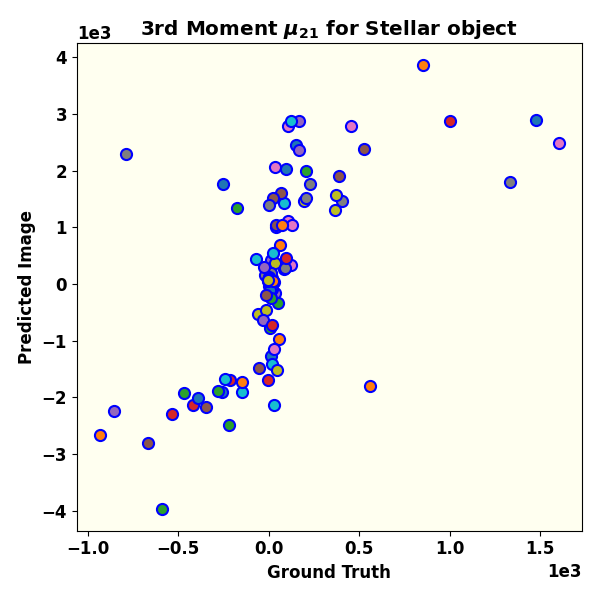
\includegraphics[width=\linewidth]{fig/moments/mom8.png}
		\caption{The 3rd order moment $\mu_{21}$.}
		\label{fig:mom9}
	\end{subfigure}\hfill
	\begin{subfigure}{0.50\linewidth}
		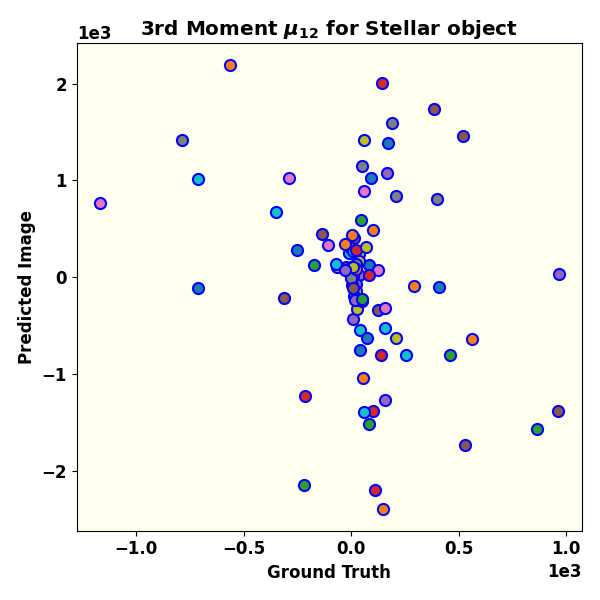
\includegraphics[width=\linewidth]{fig/moments/mom9.png}
		\caption{The 3rd order moment $\mu_{12}$.}
		\label{fig:mom10}
	\end{subfigure}\hfill
	\caption{This set of figures shows all the 3rd-order central moments for ground truth and predicted images generated by trained GAN. It calculates the skewness and evaluates the brightness distribution of images.}
	\label{fig:moments}
\end{figure*}



First, Salt and Pepper noise is introduced at a rate of \(\alpha\) (usually 0.5\%). Then, the images are resized and their mean is subtracted. A two-dimensional Fast Fourier Transform, along with a Fourier shift, is applied, yielding a complex number for each pixel. Since II does not measure phase, the absolute value is calculated (as shown in Fig.~\ref{fig:ft} on both linear and logarithmic scales for visualization). 

Next, sparse sampling is introduced via pixel-wise multiplication between the absolute-valued Fourier-transformed image (Fig.~\ref{fig:ft}) and the sparse sampling map (Fig.~\ref{fig:base}). The result is a map in the Fourier plane featuring several ellipses, which is also referred to as the sparse sampling map (Fig.~\ref{fig:ft_base}). This map represents the sparse sampling for Fig.~\ref{fig:image}, corresponding to the source observed with four telescopes (Fig.~\ref{fig:teles}). 

Finally, the pixels are normalized and converted to 8-bit integers. This image represents the sparsely sampled complex visibility as it can be measured with II. The image shown in Fig.~\ref{fig:ft_base} serves as the input for the GAN, which also requires the corresponding ground truth image. Consequently, the simulated stars are resized using the same algorithm and converted to 8-bit integers to reduce bias. The GAN must have access to the ground truth corresponding to each input image; therefore, the input and ground truth images are merged side-by-side (as shown in Fig.~\ref{fig:GANinput}) and used to train the GAN. This procedure is applied to all simulated stars, with 10\% used as test data, 10\% as validation data, and the remaining 80\% as training data.


\subsection{GAN Architecture}
The GAN used in this work is based on pix2pix, which utilizes a conditional GAN (cGAN) as discussed in the previous section \cite{isola2017image}. This architecture is highly robust and has already been applied to various problems. For instance, the TensorFlow tutorials\footnote{\url{https://www.tensorflow.org/tutorials/generative/pix2pix}} demonstrate its application to a dataset of architectural facades. However, to adapt the pix2pix GAN for the phase retrieval problem, some modifications are necessary. The network is implemented using the TensorFlow library \cite{abadi2016tensorflow}, calculations are performed with scipy \cite{virtanen2020scipy}, and plots are generated with matplotlib \cite{4160265}.

\subsection{Hyperparameter Tuning}
The GAN used in this work depends on several parameters, which are explained briefly below (for a more in-depth discussion, see \cite{murphy2022probabilistic}).

The learning rate of the optimizer determines how much the model updates its parameters with each iteration. A learning rate that is too small may lead to underfitting, while one that is too large can render the model unstable. Therefore, selecting an appropriate learning rate is crucial \cite{murphy2022probabilistic}. Figure~\ref{fig:Plot_learning_rate_loss} illustrates the effect of different learning rates on both the Generator and Discriminator losses. As expected, lower learning rates result in fewer outliers in the loss functions, indicating more stable updates. Although all models eventually stabilize at a similar level, lower learning rates are preferred.

The kernel size refers to the dimensions of the convolutional kernel used in the network, determining how many pixels are combined to produce a new pixel. A larger kernel size can capture features spanning several pixels, but it may also incorporate unrelated features. As shown in Figure~\ref{fig:Plot_kernel_size_loss}, the kernel size does not have a significant impact on the loss functions; however, smaller kernel sizes tend to produce more outliers, suggesting that either the Generator or Discriminator may gain an advantage. Therefore, a kernel size of 5 is preferred.

The amount of noise is controlled by two parameters, \(\alpha\) and \(\beta\), which indicate the percentage of pixels altered to either black or white—hence the term Salt and Pepper noise. Here, \(\alpha\) is applied to the real image, while \(\beta\) is applied to the generated image. Different ratios \(\frac{\alpha}{\beta}\) can lead to varying model performance; however, our results indicate that distinct noise rates do not significantly affect the loss functions. Figure~\ref{fig:Plot_noise_loss} shows the loss functions for smaller images (64 × 64), and due to the negligible impact, this analysis was not repeated for larger images.

The batch size defines the number of images processed simultaneously by the network. Smaller batch sizes have been observed to improve generalization \cite{prince2023understanding}. As illustrated in Figure~\ref{fig:Plot_batchsize_loss}, processing two images at once results in fewer outliers. However, because a larger batch size significantly increases training time, a batch size of 1 is used.

When training GANs, one strategy to potentially boost performance is to give the Discriminator an advantage by increasing its number of training steps before returning to the Generator's training. While this can lower the Discriminator loss—as shown in Figure~\ref{fig:Plot_discrep_loss}—it also increases training time and leads to a slight rise in the Generator loss. Since the generated images do not noticeably improve with additional Discriminator training, both networks are typically trained with the same number of steps.

Finally, the degree of sparse sampling can be varied to provide the model with access to more pixels. Increasing the number of telescopes results in more baselines and, consequently, more available pixels. Figure~\ref{fig:Plot_telescopes_loss} shows the loss functions for different numbers of telescopes. There is a significant disparity in performance, partly because the relationship between telescopes and baselines is not linear. For example, the Fourier plane can be sampled sixfold when using four telescopes compared to using only two. In the case of two telescopes, both the Generator and Discriminator exhibit less smooth training, as indicated by the outliers. Performance improves with three telescopes and becomes very promising with four. Overall, the degree of sparse sampling appears to have the most pronounced effect of all the hyperparameters.